\section{Deconvolution}\label{section:deconvolution}

The idea of Deconvolution \cite{zeiler2013visualizing} comes from the work of Zeiler et al. \cite{zeiler2011adaptive} about \textit{Deconvolutional Networks (\textit{deconvnets}}. Deconvnets are designed to work similar to convolutional networks but reverse (reversing pooling component, reversing filter component etc.), and they can be trained using an unsupervised approach. In a deconvolutional approach to explaining the model, we are not training a deconvnet but rather probe our CNN with it. 

\begin{wrapfigure}{R}{0.4\textwidth}
\vspace{-1.5\baselineskip}
\centering
  \setlength{\belowcaptionskip}{12pt}
  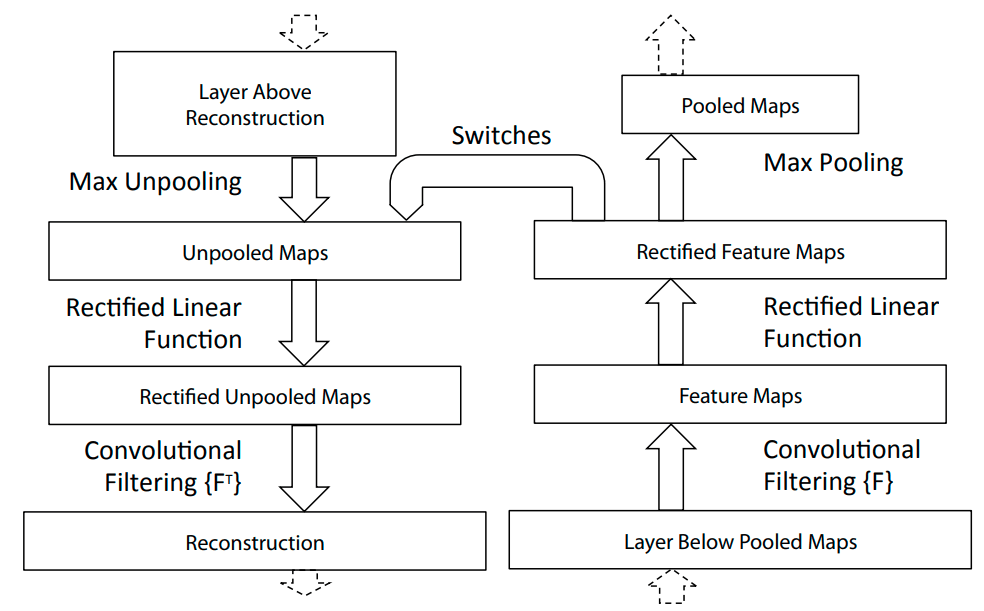
\includegraphics[width=0.4\textwidth]{methods/images/deconv-layer.png}
  \caption{A deconvnet layer (left) attached to a CNN layer (right), source \cite{zeiler2013visualizing}}\label{fig:deconvolution-layer}
  \setlength{\belowcaptionskip}{12pt}
  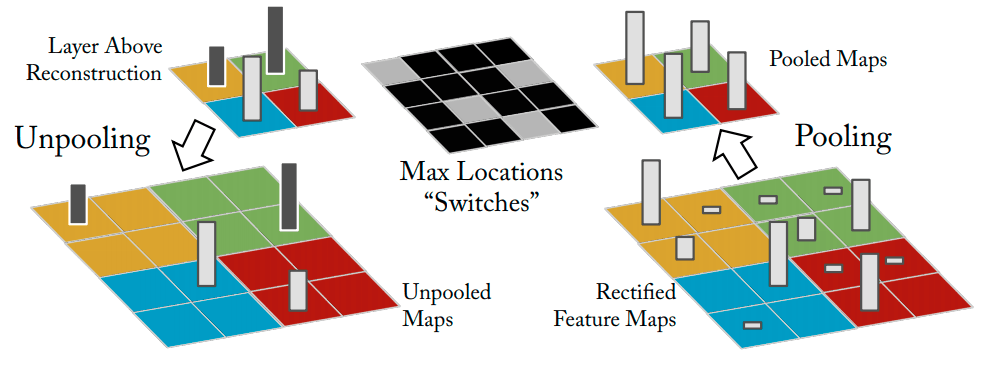
\includegraphics[width=0.4\textwidth]{methods/images/deconv-layer-unpooling.png}
  \caption{The unpooling layer, source \cite{zeiler2013visualizing}}\label{fig:deconvolution-layer-unpooling}
  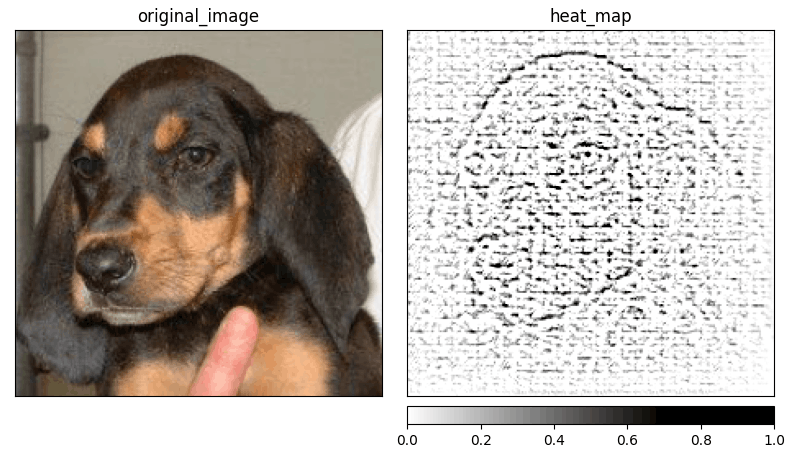
\includegraphics[width=0.35\textwidth]{methods/images/deconv-black-and-tan-coonhound.png}
  \caption{Visualization of the saliency map generated by deconvolution for the class \textit{black-and-tan-coonhound}. Image source: \textit{Stanford Dogs} \cite{stanford-dogs}}\label{fig:saliency-map-coonhound}
    \vspace{-\baselineskip}
\end{wrapfigure}

\vspace{\baselineskip}

To reconstruct the activation on a specific layer, we are attaching \textit{deconv layers} to corresponding \textit{CNN layers} (see Fig. \ref{fig:deconvolution-layer}). Then an image is passed through the CNN, and the network computes the output. To examine a reconstruction for a given class $c$, we have to set all activations except the one responsible for predicting class $c$ to zero. Then we can propagate through deconvnet layers and pass all the feature maps as inputs to corresponding layers.

\vspace{\baselineskip}

To calculate the reconstruction, deconvnet layer has to be able to reverse operations performed by the CNN layers. Authors designed specific components to compote the reverse operations done by CNN layers:

\vspace{\baselineskip}

\textbf{Filtering} in the original CNN computes \textit{feature maps} using learned filters. Reversing that operation requires the use of a transposed version of the same filters. Those transposed filters are then applied to the \textit{Rectified Unpooled Maps}.

\vspace{\baselineskip}


\textbf{Rectification} uses the same \textit{ReLU} non-linearity \cite{hahnloser2000digital} to compute \textit{Rectified Unpooled Maps} as it is used in CNN. It is simply just rectifying the values and propagate only non-negative ones to the \textit{filtering} layer.

\vspace{\baselineskip}

\textbf{Unpooling} corresponds to the \textit{Pooling Layer} of CNN (see Fig. \ref{fig:deconvolution-layer-unpooling}). The original max-pooling operation is non-invertible, but this approach uses additional variables called \textit{switch variables}, which are responsible for remembering the locations of the maxima for each pooling region. The unpooling layer uses these variables to make a reconstruction into the same locations as when the pooling was calculated.

\vspace{\baselineskip}

Propagation through the whole deconvnet gives us a representation of the features from the first layer of the original CNN (the last deconvnet layer corresponds to the first CNN layer). This approach causes the saliency map to feature some biases from the first convolutional layer and the representation looks like a localized edge detector (see Fig. \ref{fig:saliency-map-coonhound}). It usually works better when there is a clear distinction in the feature importance rather than similar values for the whole image.